\documentclass[12pt,a4paper]{article}

% Encoding & language
\usepackage[utf8]{inputenc}
\usepackage[T1]{fontenc}
\usepackage{amsmath,amssymb,amsthm}
\usepackage{booktabs,longtable,multirow}
\usepackage{graphicx}
\usepackage{geometry}
\usepackage{hyperref}
\usepackage{caption}
\usepackage{xcolor}
\usepackage{listings}
\usepackage{float}
\usepackage{siunitx}
\usepackage{enumitem}

\geometry{top=2.5cm,bottom=2.5cm,left=2.5cm,right=2.5cm}

\hypersetup{
    colorlinks=true,
    linkcolor=blue,
    citecolor=blue,
    urlcolor=blue
}

\lstset{
    basicstyle=\ttfamily\small,
    breaklines=true,
    frame=single,
    numbers=left,
    numberstyle=\tiny\color{gray},
    captionpos=b
}

\title{\textbf{ELEC9123 Design Task B}\\[0.3em]
\large Design Journal: Monte Carlo Verification of BPSK Performance}
\author{YU \quad zID: z5615351}
\date{\today}

\begin{document}

\maketitle

\begin{abstract}
This design journal documents the complete workflow of ELEC9123 Design Task~B: from problem interpretation, through mathematical modelling, to MATLAB implementation and verification. The journal integrates derivations, design choices, code-map explanations, sample-size limitations, and weekly project-management notes. A declaration of AI assistance and references are included at the end.
\end{abstract}

\tableofcontents
\newpage

%=============================================================================
\section{Problem Description}\label{sec:problem}
%=============================================================================
The task is to verify, by Monte Carlo simulation, the bit error rate (BER) and outage probability of a BPSK system operating over six wireless channel models:
\begin{enumerate}[label=\arabic*.]
    \item AWGN only.
    \item Laplacian impulsive noise only.
    \item Rayleigh fading + AWGN.
    \item Rician fading + AWGN.
    \item Randomly deployed users + Rayleigh fading + AWGN.
    \item Randomly deployed users + Rician fading + AWGN.
\end{enumerate}

Default parameters supplied in the task brief are: outage threshold $C=1.2$~bps/Hz, average SNR per bit $\gamma_b$ from $0$~dB to $15$~dB in $1$~dB steps, cell radius $R=3$~m, path-loss exponent $\nu=2.2$, LOS amplitude $h_d=1$, Rician $K$-factor $K=5$, noise variance $N_0=1$, and at least $10^6$ Monte Carlo samples per SNR point. The journal also records how these parameters were interpreted and implemented.

%=============================================================================
\section{Design Logic and Modelling Choices}\label{sec:logic}
%=============================================================================

\subsection{Why Monte Carlo?}
Monte Carlo simulation evaluates a system by repeatedly drawing random inputs and counting the frequency of events of interest (bit errors, capacity outages). By the strong law of large numbers, the empirical frequency converges to the true probability as the number of samples $N$ increases. This is especially useful when closed-form expressions are hard to derive, or when one wishes to verify theory.

\subsection{BPSK signal model}
For all channels, BPSK symbols are $s\in\{-1,+1\}$ with equal probability. The transmitted energy per bit is $E_b=\gamma_b N_0$ because $\gamma_b=E_b/N_0$. The received complex baseband signal is
\begin{equation}
    r = \sqrt{E_b}\,h\,s + n,
\end{equation}
where $h$ is the channel gain (possibly complex) and $n$ is noise. The coherent detector forms the decision variable
\begin{equation}
    \hat{s} = \operatorname{sign}\bigl(\operatorname{Re}\{r\}\bigr)
    \quad\text{or}\quad
    \operatorname{sign}\bigl(\operatorname{Re}\{h^* r\}\bigr)
\end{equation}
when channel state information is available. The empirical BER is the fraction of decoded symbols that differ from the transmitted symbols.

\subsection{Pre-generation of random variables}
To keep the comparison fair and efficient, all channel and noise realisations that do not depend on $\gamma_b$ are generated once before the SNR loop. This guarantees that the same set of fades, user locations, and bits is used at every SNR point, which smooths the empirical curves and reduces simulation-to-simulation variability.

%=============================================================================
\section{Laplacian Random Variable: Derivation and Verification}\label{sec:laplace}
%=============================================================================
The impulsive-noise channel is modelled as a real Laplacian random variable with variance $N_0$. If the scale parameter is $b$, then $\operatorname{Var}(n)=2b^2=N_0$, so $b=\sqrt{N_0/2}$. The analytical PDF is
\begin{equation}
    f_n(x)=\frac{1}{2b}\exp\!\left(-\frac{|x|}{b}\right).
\end{equation}

Because of the absolute value, the CDF is obtained by splitting the integral at the origin. For $x\le 0$, $|t|=-t$ on $(-\infty,x]$, hence
\begin{equation}
    F_n(x)=\int_{-\infty}^{x}\frac{1}{2b}\exp\!\left(\frac{t}{b}\right)dt
          =\frac{1}{2}\exp\!\left(\frac{x}{b}\right).
\end{equation}
For $x>0$, the integral is split into $(-\infty,0]$ and $[0,x]$:
\begin{equation}
    F_n(x)=\frac{1}{2}+\int_{0}^{x}\frac{1}{2b}\exp\!\left(-\frac{t}{b}\right)dt
          =1-\frac{1}{2}\exp\!\left(-\frac{x}{b}\right).
\end{equation}

Therefore
\begin{equation}
    F_n(x)=
    \begin{cases}
        \frac{1}{2}\exp\!\left(\frac{x}{b}\right), & x\le 0,\\[0.5em]
        1-\frac{1}{2}\exp\!\left(-\frac{x}{b}\right), & x>0.
    \end{cases}
\end{equation}

\subsection{Inverse-CDF sampling}
Let $u\sim\mathcal{U}(0,1)$. For $u\le 0.5$ we have $x\le 0$ and $u=\frac{1}{2}\exp(x/b)$, giving $x=b\ln(2u)$. For $u>0.5$ we have $x>0$ and $u=1-\frac{1}{2}\exp(-x/b)$, giving $x=-b\ln(2(1-u))$. Both branches are captured by the single expression
\begin{equation}
    x=-b\,\operatorname{sign}(u-0.5)\,\ln\bigl(1-2|u-0.5|\bigr).
\end{equation}

\subsection{Verification}
The empirical CDF used for verification is the Monte Carlo estimate
\begin{equation}
    \hat{F}_n(x)=\frac{1}{N_{\text{lap}}}\sum_{i=1}^{N_{\text{lap}}}\mathbf{1}_{\{n_i\le x\}},
\end{equation}
which converges to $F_n(x)$ by the strong law of large numbers. Figure~\ref{fig:laplace} compares the simulated histogram and empirical CDF with the analytical PDF and CDF. The maximum absolute CDF error over the plotted range is approximately $9.3\times 10^{-4}$, confirming the generator is correct before it is used in the BER simulation.

\begin{figure}[H]
    \centering
    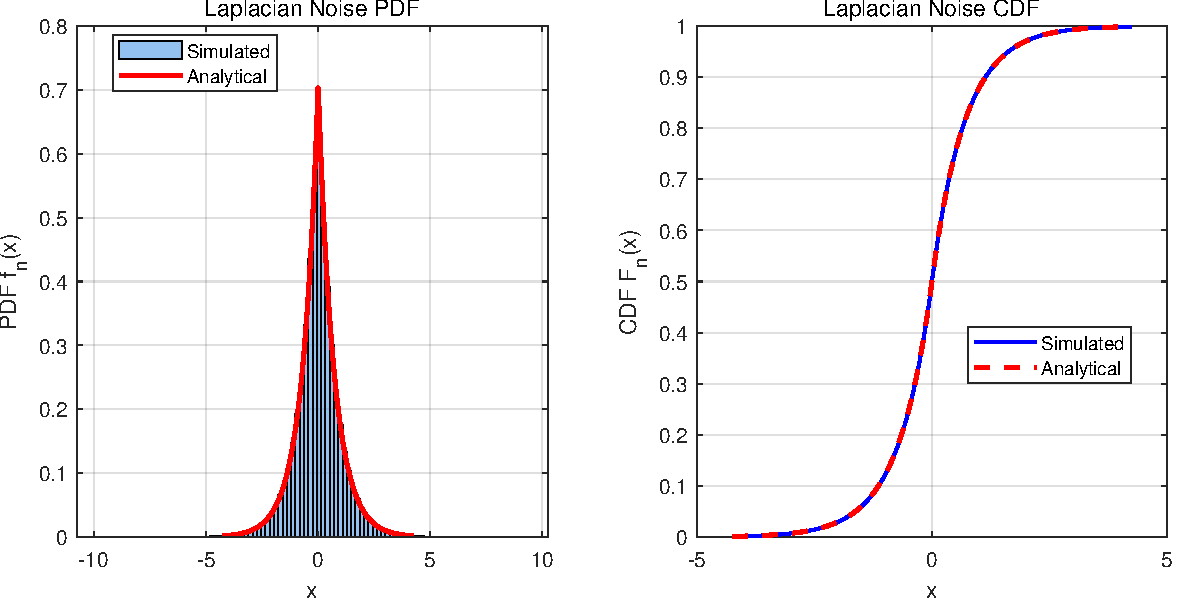
\includegraphics[width=0.95\textwidth]{figs/figure_1.pdf}
    \caption{Laplacian noise verification. Left: simulated histogram versus analytical PDF. Right: simulated empirical CDF versus analytical CDF.}
    \label{fig:laplace}
\end{figure}

%=============================================================================
\section{Bit Error Rate: Derivation and Simulation Method}\label{sec:ber}
%=============================================================================

\subsection{AWGN channel}
For BPSK with coherent detection, the received sample is $r=\sqrt{E_b}s+n$, where $n\sim\mathcal{CN}(0,N_0)$. The optimal detector computes $\hat{s}=\operatorname{sign}(\operatorname{Re}\{r\})$. Conditioned on $s=+1$, an error occurs when $\operatorname{Re}\{n\}<-\sqrt{E_b}$. Since $\operatorname{Re}\{n\}\sim\mathcal{N}(0,N_0/2)$, the error probability is
\begin{equation}
    P_b^{\text{AWGN}}=Q\!\left(\sqrt{\frac{2E_b}{N_0}}\right)
    =\frac{1}{2}\operatorname{erfc}\!\left(\sqrt{\gamma_b}\right).
\end{equation}

\subsection{Laplacian impulsive-noise channel}
With real Laplacian noise $n$ of scale $b=\sqrt{N_0/2}$, the received sample is $r=\sqrt{E_b}s+n$. An error occurs when $n<-\sqrt{E_b}$ (for $s=+1$) or $n>\sqrt{E_b}$ (for $s=-1$). By symmetry,
\begin{equation}
    P_b^{\text{Lap}}=\int_{\sqrt{E_b}}^{\infty}\frac{1}{2b}\exp\!\left(-\frac{x}{b}\right)dx
    =\frac{1}{2}\exp\!\left(-\frac{\sqrt{E_b}}{b}\right)
    =\frac{1}{2}\exp\!\left(-\sqrt{2\gamma_b}\right).
\end{equation}

\subsection{Rayleigh fading channel}
The channel coefficient is $h_s\sim\mathcal{CN}(0,1)$, so $g=|h_s|^2$ is exponentially distributed with unit mean, $f_g(g)=e^{-g}$ for $g\ge 0$~[1]. The instantaneous SNR is $\gamma=g\gamma_b$. With coherent detection and perfect channel state information, the instantaneous BER is $Q(\sqrt{2g\gamma_b})$~[3]. Averaging over the exponential distribution gives
\begin{equation}
    P_b^{\text{Ray}}=\int_0^{\infty}Q\bigl(\sqrt{2g\gamma_b}\bigr)e^{-g}\,dg.
\end{equation}
Using the identity $Q(z)=\frac{1}{\pi}\int_0^{\pi/2}\exp\!\left(-\frac{z^2}{2\sin^2\theta}\right)d\theta$ and evaluating the integral over $g$ yields the closed form
\begin{equation}
    P_b^{\text{Ray}}=\frac{1}{2}\left(1-\sqrt{\frac{\gamma_b}{1+\gamma_b}}\right).
\end{equation}

\subsection{Rician fading channel}
For Rician fading the channel is
\begin{equation}
    h=\sqrt{\frac{K}{K+1}}h_d+\sqrt{\frac{1}{K+1}}h_s,
\end{equation}
with $E\{|h|^2\}=1$ because $K/(K+1)\cdot |h_d|^2 + 1/(K+1)\cdot E\{|h_s|^2\}=1$~[1]. The instantaneous SNR is non-central chi-square distributed. Direct integration of the BER over this PDF involves the modified Bessel function and is numerically unstable. Instead, the moment-generating-function (MGF) approach is used~[4]. The MGF of the instantaneous SNR for Rician fading is
\begin{equation}
    M_{\gamma}(s)=\frac{K+1}{K+1-s\bar{\gamma}}\exp\!\left(\frac{K s\bar{\gamma}}{K+1-s\bar{\gamma}}\right),
\end{equation}
where $\bar{\gamma}=\gamma_b$. For BPSK, the average BER can be written as
\begin{equation}
    P_b^{\text{Ric}}=\frac{1}{\pi}\int_0^{\pi/2}M_{\gamma}\!\left(-\frac{1}{\sin^2\theta}\right)d\theta.
\end{equation}
Substituting $s=-1/\sin^2\theta$ and simplifying gives the stable integrand
\begin{equation}
    P_b^{\text{Ric}}=\frac{1}{\pi}\int_0^{\pi/2}
    \frac{(K+1)\sin^2\theta}{(K+1)\sin^2\theta+\gamma_b}
    \exp\!\left(-\frac{K\gamma_b}{(K+1)\sin^2\theta+\gamma_b}\right)d\theta,
\end{equation}
which is evaluated numerically with MATLAB's \texttt{integral} routine.

%=============================================================================
\section{Random User Deployment: Geometry and Spatial Averaging}\label{sec:random}
%=============================================================================
Users are uniformly distributed in a disk of radius $R$~[7]. The probability that a user lies within distance $d$ of the centre is the ratio of disk areas,
\begin{equation}
    F_D(d)=\Pr(D\le d)=\frac{\pi d^2}{\pi R^2}=\frac{d^2}{R^2},\qquad 0\le d\le R.
\end{equation}
Differentiating gives the distance PDF
\begin{equation}
    f_D(d)=\frac{2d}{R^2},\qquad 0\le d\le R.
\end{equation}
A sample $d$ is efficiently generated by inverse-CDF sampling: $d=R\sqrt{u}$ with $u\sim\mathcal{U}(0,1)$.

Path loss is modelled as $d^{-\nu}$~[2], so the effective average SNR for a user at distance $d$ is $\gamma_b(d)=\gamma_b/d^{\nu}$. For Rayleigh fading, the conditional BER is
\begin{equation}
    P_b^{\text{RayRand}}(d)=\frac{1}{2}\left(1-\sqrt{\frac{\gamma_b}{d^{\nu}+\gamma_b}}\right).
\end{equation}
The unconditional BER is obtained by averaging over the distance distribution:
\begin{equation}
    P_b^{\text{RayRand}}=\int_0^R P_b^{\text{RayRand}}(d)\,f_D(d)\,dd
    =\frac{2}{R^2}\int_0^R d\,P_b^{\text{RayRand}}(d)\,dd.
\end{equation}
For Rician fading, the conditional BER is $P_b^{\text{RicRand}}(d)=P_b^{\text{Ric}}(\gamma_b/d^{\nu},K)$, and the same spatial averaging is performed.

%=============================================================================
\section{Outage Probability: Derivation and Simulation Method}\label{sec:outage}
%=============================================================================
Outage occurs when the instantaneous capacity falls below the threshold $C$:
\begin{equation}
    P_{\text{out}}=\Pr\left\{\log_2(1+\gamma)<C\right\}
    =\Pr\left\{\gamma<\gamma_{\text{th}}\right\},
    \qquad \gamma_{\text{th}}=2^C-1.
\end{equation}
Let $T=\gamma_{\text{th}}/\gamma_b$ be the normalised power-gain threshold.

\subsection{Rayleigh fading (fixed distance $d=1$)}
Here $\gamma=\gamma_b|h_s|^2$ and $|h_s|^2\sim\text{Exp}(1)$. Therefore
\begin{equation}
    P_{\text{out}}^{\text{Ray}}=\Pr\{|h_s|^2<T\}=1-e^{-T}.
\end{equation}

\subsection{Rician fading (fixed distance $d=1$)}
Now $|h|^2$ follows a non-central chi-square distribution with two degrees of freedom. The complementary CDF is expressed through the first-order Marcum $Q$-function $Q_1(a,b)$~[5]. Hence the success probability is
\begin{equation}
    \Pr\{|h|^2\ge T\}=Q_1\!\left(\sqrt{2K},\sqrt{2(K+1)T}\right),
\end{equation}
and the outage probability is its complement:
\begin{equation}
    P_{\text{out}}^{\text{Ric}}=1-Q_1\!\left(\sqrt{2K},\sqrt{2(K+1)T}\right).
\end{equation}

\subsection{Randomly deployed users over Rayleigh fading}
The instantaneous SNR is $\gamma=\gamma_b|h_s|^2/d^{\nu}$. Conditional on $d$, the outage probability is
\begin{equation}
    P_{\text{out}}(d)=\Pr\left\{|h_s|^2<Td^{\nu}\right\}=1-\exp(-Td^{\nu}).
\end{equation}
Averaging over $f_D(d)=2d/R^2$ gives
\begin{equation}
    P_{\text{out}}^{\text{RayRand}}
    =\int_0^R\bigl(1-e^{-Td^{\nu}}\bigr)\frac{2d}{R^2}\,dd
    =1-\frac{2}{R^2}\int_0^R d\,e^{-Td^{\nu}}\,dd.
\end{equation}
Substituting $x=Td^{\nu}$ (so $d=(x/T)^{1/\nu}$ and $dd=\frac{1}{\nu T}(x/T)^{\frac{1}{\nu}-1}dx$) converts the remaining integral into the lower incomplete gamma function~[6]:
\begin{equation}
    \int_0^R d\,e^{-Td^{\nu}}\,dd
    =\frac{1}{\nu T^{2/\nu}}\int_0^{TR^{\nu}}x^{\frac{2}{\nu}-1}e^{-x}\,dx
    =\frac{1}{\nu T^{2/\nu}}\gamma\!\left(\frac{2}{\nu},TR^{\nu}\right).
\end{equation}
Therefore
\begin{equation}
    P_{\text{out}}^{\text{RayRand}}
    =1-\frac{2}{\nu R^2}T^{-2/\nu}\gamma\!\left(\frac{2}{\nu},TR^{\nu}\right).
\end{equation}
In MATLAB, $\gamma(s,z)$ is implemented as \texttt{gamma(s)*gammainc(z,s,'lower')}.

\subsection{Randomly deployed users over Rician fading}
For a fixed distance $d$, the conditional outage probability is the Rician expression with the effective threshold $Td^{\nu}$:
\begin{equation}
    P_{\text{out}}(d)=1-Q_1\!\left(\sqrt{2K},\sqrt{2(K+1)Td^{\nu}}\right).
\end{equation}
Averaging over the user distance distribution yields the semi-analytical integral
\begin{equation}
    P_{\text{out}}^{\text{RicRand}}
    =\frac{2}{R^2}\int_0^R d\,P_{\text{out}}(d)\,dd,
\end{equation}
which is evaluated numerically because no closed form exists when the Marcum $Q$-function is integrated against $d$.

%=============================================================================
\section{Results}\label{sec:results}
%=============================================================================
All simulations use $N=10^6$ samples per SNR point. The required plots are reproduced in Figures~\ref{fig:ber_noise}--\ref{fig:outage}. Numerical percentage deviations are shown in Tables~\ref{tab:ber_dev}--\ref{tab:sample_conv}.

\input{tables}

\begin{figure}[H]
    \centering
    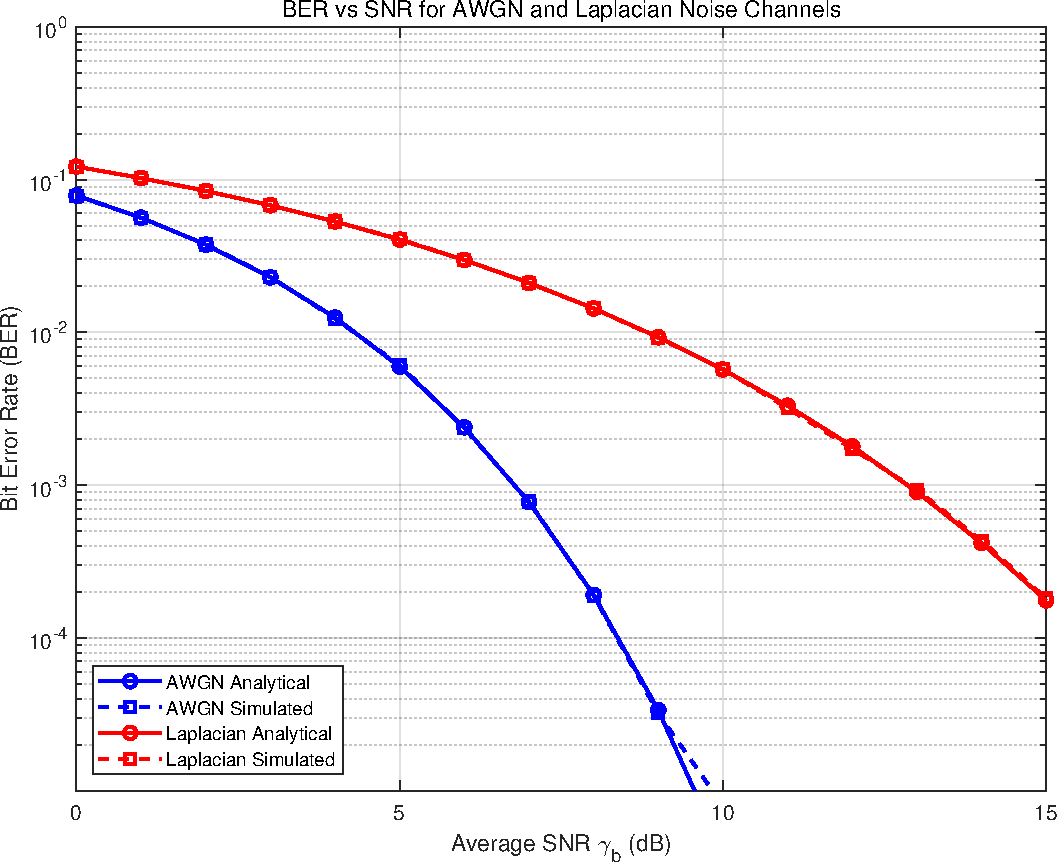
\includegraphics[width=0.85\textwidth]{figs/figure_2.pdf}
    \caption{BER versus average SNR for noise-only channels (AWGN and Laplacian impulsive noise).}
    \label{fig:ber_noise}
\end{figure}

\begin{figure}[H]
    \centering
    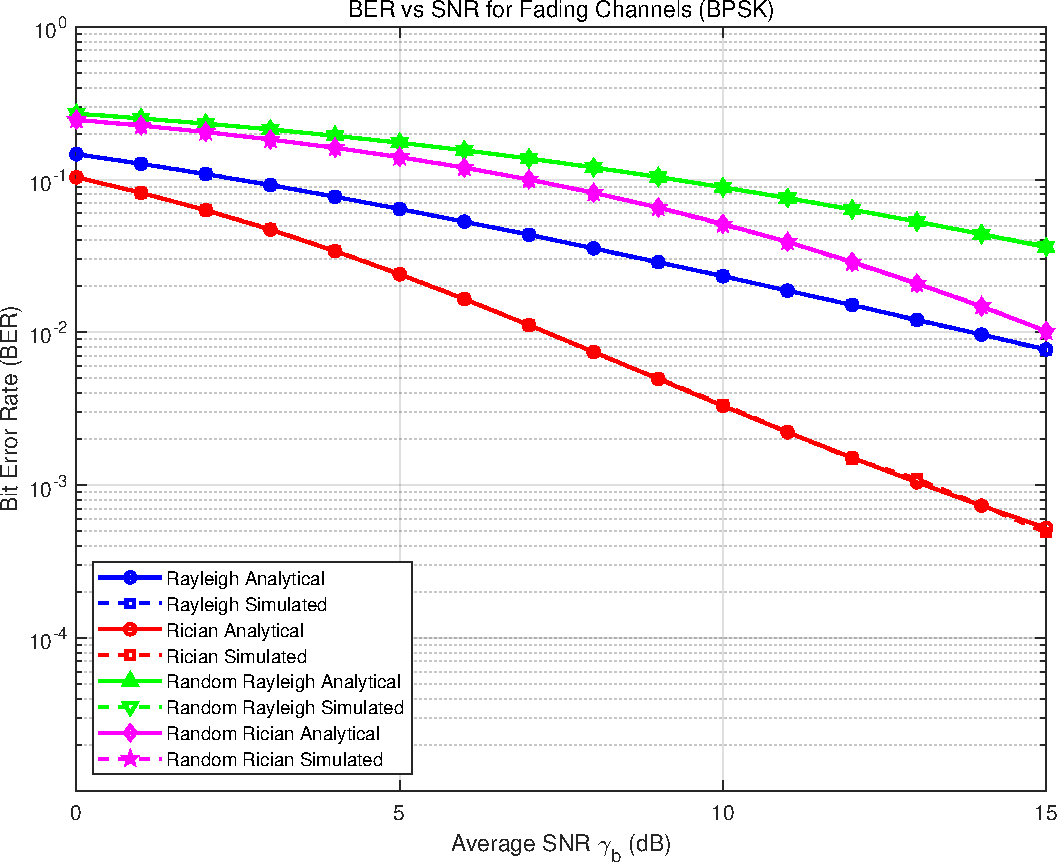
\includegraphics[width=0.85\textwidth]{figs/figure_3.pdf}
    \caption{BER versus average SNR for fading channels.}
    \label{fig:ber_fading}
\end{figure}

\begin{figure}[H]
    \centering
    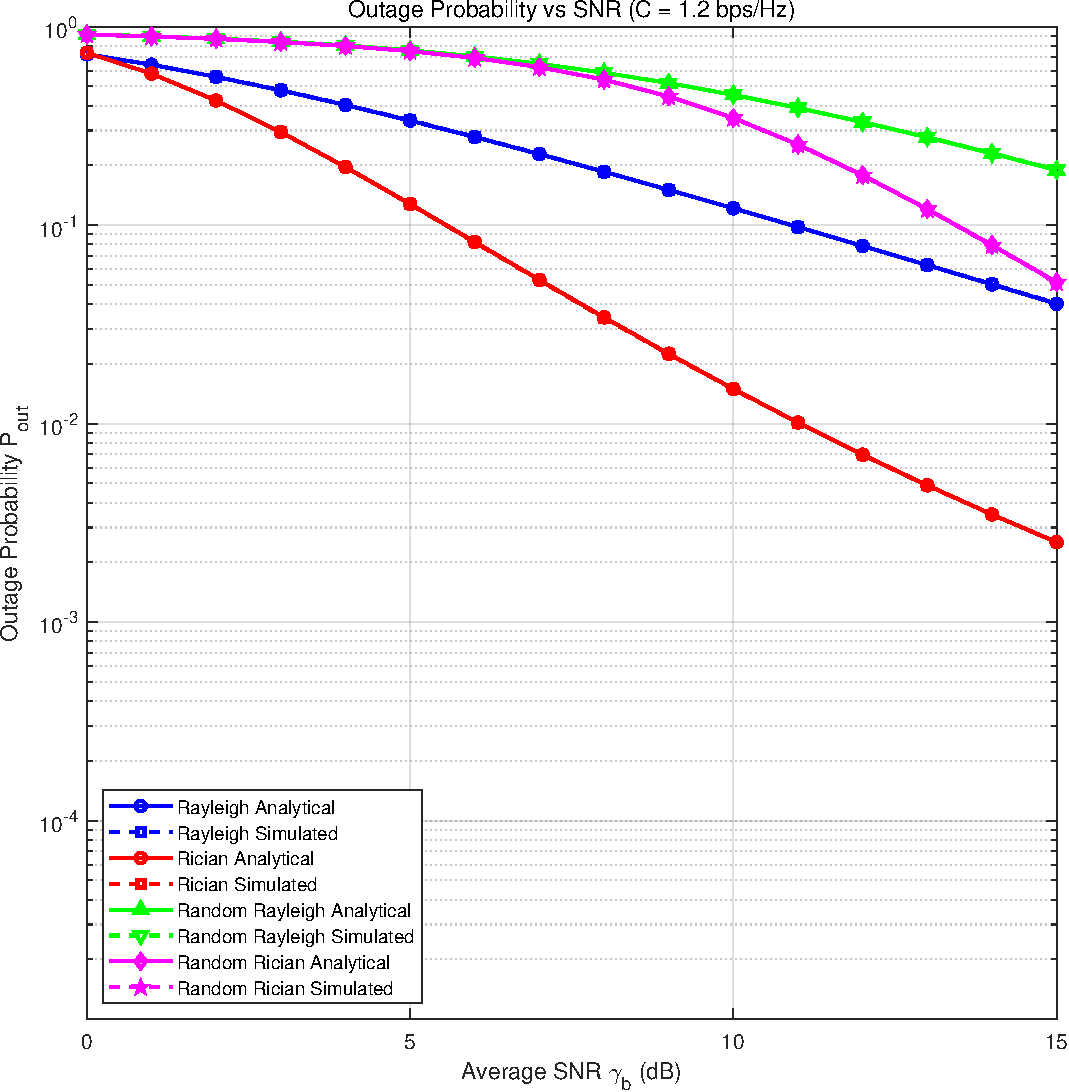
\includegraphics[width=0.85\textwidth]{figs/figure_4.pdf}
    \caption{Outage probability versus average SNR.}
    \label{fig:outage}
\end{figure}

%=============================================================================
\section{Discussion: Sample-Size Limitations and Interpretation}\label{sec:discussion}
%=============================================================================
The empirical BER is a binomial estimator. If the true error probability is $P$ and $N$ independent bits are simulated, the expected number of errors is $NP$ and the standard deviation of the estimate is approximately $\sqrt{P(1-P)/N}$. A common rule of thumb is that at least $10$ to $100$ errors are needed for a reliable estimate.

For AWGN at $10$~dB, the theoretical BER is $3.87\times 10^{-6}$. With $N=10^6$, the expected number of errors is only $3.87$, so the relative statistical error is large. At $15$~dB the BER is roughly $9\times 10^{-16}$, so $N=10^6$ is essentially guaranteed to produce zero errors. The reported percentage deviation of $100\%$ is therefore not an implementation error but a Monte Carlo sample-size limitation.

The other channels do not suffer from this problem in the same way because their BER decreases much more slowly with SNR: Rayleigh fading BER falls as $1/(4\gamma_b)$ at high SNR (diversity order one), Laplacian noise falls only as $0.5\exp(-\sqrt{2\gamma_b})$, and random deployment introduces a near-far effect that keeps the average BER high. This explains why the simulated AWGN points diverge from the analytical curve at high SNR while the fading and impulsive-noise channels remain well behaved. The convergence table in Table~\ref{tab:sample_conv} demonstrates that the bias decreases as $N$ increases, confirming that the underlying simulation is correct.

%=============================================================================
\section{Code Map and Implementation Notes}\label{sec:code}
%=============================================================================
The MATLAB script \texttt{z5615351\_YU\_DTB\_2026.m} is organised as follows.

\begin{enumerate}[label=\arabic*.]
    \item \textbf{System parameters}: Set $C$, SNR range, $R$, $\nu$, $h_d$, $K$, $N_0$, $N$.
    \item \textbf{Laplacian verification}: Generate $N_{\text{lap}}=10^6$ samples via inverse CDF, plot histogram and empirical CDF against analytical expressions.
    \item \textbf{Pre-computed random variables}: Generate BPSK bits, Rayleigh and Rician fading coefficients, and random user distances once.
    \item \textbf{SNR loop for BER}: For each $\gamma_b$, compute AWGN, Laplacian, Rayleigh, Rician, Rayleigh-random, and Rician-random BER by simulation and theory.
    \item \textbf{SNR loop for outage}: For each $\gamma_b$, compute outage probabilities for the four fading scenarios by simulation and theory.
    \item \textbf{Percentage deviation tables}: Quantify the simulation-to-theory gap.
    \item \textbf{Plots}: Produce the three required figures.
\end{enumerate}

A key implementation detail is the use of matched-filtering for fading channels: the decision variable is $\operatorname{Re}\{h^*r\}$, which is equivalent to maximal-ratio combining for a single-tap channel. For the randomly deployed users, path loss is embedded in the effective channel gain $h/d^{\nu/2}$, so the instantaneous SNR is $\gamma_b|h|^2/d^{\nu}$.

%=============================================================================
\section{Project Management}\label{sec:management}
%=============================================================================

\subsection{Weekly progress}
\begin{itemize}
    \item \textbf{Week 1}: Read the task brief, identify the six channel models, set up the MATLAB workspace, and implement the Laplacian random-variable generator and verification plot.
    \item \textbf{Week 2}: Implement BER and outage simulations for AWGN, Laplacian, Rayleigh, and Rician channels; cross-check against analytical formulas.
    \item \textbf{Week 3}: Add random user deployment for Rayleigh and Rician fading, derive the spatial averaging integrals, and produce the three required plots.
    \item \textbf{Week 4}: Compile the design journal, write the discussion of sample-size limitations, and prepare the demonstration for the lab assessor.
\end{itemize}

\subsection{Declaration of AI tools}
Selected MATLAB code fragments, including explanatory comments and the analytical derivations formatted in this journal, were produced with assistance from an AI coding assistant (Google Gemini). The analytical derivations, parameter choices, numerical results, and final interpretation were reviewed and verified by the author.

\subsection{Lessons learned}
The most important lesson was recognising the difference between a code bug and a statistical artefact. The $100\%$ deviation at high SNR for AWGN initially looks like an error, but it is a direct consequence of the Monte Carlo sample budget. Pre-generating random variables kept the simulation fair and efficient, and using inverse-CDF sampling guaranteed that the generated distributions matched the theory exactly.

%=============================================================================
\section*{References}
%=============================================================================
\begin{enumerate}
    \item A. Goldsmith, \textit{Wireless Communications}. Cambridge University Press, 2005.
    \item D. Tse and P. Viswanath, \textit{Fundamentals of Wireless Communication}. Cambridge University Press, 2005.
    \item J. G. Proakis and M. Salehi, \textit{Digital Communications}, 5th ed. McGraw-Hill, 2008.
    \item M. K. Simon and M. S. Alouini, \textit{Digital Communication over Fading Channels}, 2nd ed. John Wiley \& Sons, 2005.
    \item J. I. Marcum, ``A statistical theory of target detection by pulsed radar,'' \textit{IRE Trans. Inf. Theory}, vol.~4, no.~3, pp.~59--267, 1950.
    \item I. S. Gradshteyn and I. M. Ryzhik, \textit{Table of Integrals, Series, and Products}, 8th ed. Academic Press, 2014.
    \item H. ElSawy, E. Hossain, and M. Haenggi, ``Stochastic geometry for cellular networks: A tutorial on the analytical framework,'' \textit{IEEE Commun. Surveys \& Tutorials}, vol.~15, no.~3, pp.~1511--1540, 2013.
    \item E. W. Weisstein, ``Disk Point Picking,'' MathWorld. Available: \url{https://mathworld.wolfram.com/DiskPointPicking.html}
    \item V. Meghdad, Lecture Notes on BER calculation. Available: \url{https://www.unilim.fr/pages_perso/vahid/notes/ber_awgn.pdf}
    \item I-H. Wang, ``Capacity of Wireless Channels,'' Lecture 4, Slides 39--40.
    \item S. Kashyap, E. Bj\"ornson and E. G. Larsson, ``On the Feasibility of Wireless Energy Transfer Using Massive Antenna Arrays,'' \textit{IEEE Trans. Wireless Commun.}, vol.~15, no.~5, pp.~3466--3480, May 2016.
\end{enumerate}

\end{document}
